\documentclass{article}

\usepackage[utf8]{inputenc}
\usepackage{natbib}
\usepackage{setspace}
\usepackage{graphicx}
\usepackage{subfig}
\usepackage{amsmath}
\usepackage{algorithm}
\usepackage[noend]{algpseudocode}
\usepackage{listings}
\usepackage{comment}
\usepackage{afterpage}
\usepackage{hyperref}
%\usepackage{fullpage}

%% BN: todonotes can be removed for final version
\usepackage[backgroundcolor=pink,linecolor=red]{todonotes}

\makeatletter
\def\BState{\State\hskip-\ALG@thistlm}
\makeatother

%\singlespacing
\onehalfspacing
%\doublespacing
%\setstretch{1.1}
\pagenumbering{roman}
\interfootnotelinepenalty=10000


\begin{document}
\linespread{1.0}

\begin{titlepage}
    \begin{center}
        \vspace*{1cm}
        
        \textbf{Speeding up the Tortoise}
        
        \vspace{0.5cm}
        A Case Study in Optimizing Forward-Moving Evolutionary Simulations
        
        \vspace{1.3cm}
        
        \textbf{Jared Galloway}
        
        \vfill
        
        
        A thesis presented for the partial fulfillment of\\
        Departmental Honors in Computer and Information Science
        
         CIS Faculty Advisor: Dr. Boyana Norris
        
        Principle Investigator: Dr. Peter Ralph
        
        \vspace{0.8cm}
        
        
\includegraphics[width=0.4\textwidth]{../figures/Oregon}
        
        %Computer and Information Science\\
        %University of Oregon\\
        Ralph Lab | HPCL
        
        June 2018
        
    \end{center}
\end{titlepage}


\section*{Acknowledgments}

Thanks to Dr. Peter Ralph for suggesting this project, helping every step of the way, and teaching me so much throughout the last year. 
Thanks to Dr. Ben Haller for giving me the opportunity to work on SLiM, lots of help, and being a great cribbage partner.
Thank you to Dr. Boyana Norris for advising and helping me structure this thesis.
Finally, thanks to my parents for the constant support throughout my college career.

This work benefited from access to the University of Oregon high-performance computer, Talapas.

\newpage

\tableofcontents
\newpage
 \setcounter{page}{1}
\pagenumbering{arabic}
\setcounter{section}{0}

%%TAKE OUT WE TO CLARIFY THE SUBJECT / AUDIENCE
%%REPLACE ALL `PEDIGREE RECORDING` with 'TREE SEQUENCE RECORDING'

%Boyana Notes -- 
%Take out dashes
% Fix quotes.
% Takes 
% Fix tense
% fix acknologements spelling

\section{Abstract}

Large-scale, forward-moving evolutionary simulations are starting to play a key role in research surrounding populations genetics. 
Simulations can help biologists understand data we observe from natural populations  
in fields such as molecular ecology, evolutionary genetics, and conservation biology.
However, the magnitude of these simulations is limited by the current capabilities of the hardware they are running on. 
This draws interest in exploring methods that make the results of large-scale simulations more feasible. 
Earlier this year, a strategy was introduced allowing simulations to avoid tracking and propagating neutral 
mutations as a consequence of storing the entire genealogical history of sampled genotypes.
In this thesis, we use succinct tree sequences, introduced by \textbf{msprime}, to
explore and implement the method of genealogical tree sequence recording (\textit{TreeSeq})
in forward-moving evolutionary simulations.
We then analyze the runtime performance gain of one to two orders of magnitude as a result of 
implementing this strategy into a popular evolutionary framework, \textbf{SLiM}.
Finally, we explain the workflow, algorithms, and data structures 
behind the implementation.

\section{Introduction}

From an evolutionary standpoint, it makes sense that the tortoise has no need to be quick.
Yet, an evolutionary biologist might wonder,
how did this adaptation come about at the genomic and ecological level? 
How important is connectivity between habitats for the tortoise?
The use of population genetics gives biologists the tools to better understand parameters including
population size, migration rates, and evolutionary history 
in fields such as molecular ecology, evolutionary genetics, and conservation biology \cite{Luikart2003}.

Commonly, science is conducted through the use of observation, analysis, and verbal hypothesis. 
To test the validity of a verbal hypothesis, one must show  ``proof of concept''|
which is where researchers would like to use mathematical models.
A key component to understanding how the evolutionary forces relate to the data sets we observe in nature
can be further analyzed through the use of theoretical evolutionary models. 
Population genetics often makes progress by gaining an understanding
of the behavior underlying models, then observing 
nature to compare whether the models are compatible \cite{gillespie2004}.

When attempting to model realistic evolutionary dynamics, 
the use of large-scale, forward-moving simulations is becoming increasingly popular \cite{Hoban}. 
Simulations have the ability to capture the underlying impact of dynamic population sizes, migration rates, and geography 
on various evolutionary forces throughout 
ecological timescales\footnote{Timescales on which we can see the impact of ecological processes such as evolution}.
Evolutionary simulations are a powerful tool when there is some map connecting the parameters we want to learn about
and the genetic data we observe in nature. 
Without knowledge of what that map is, simulations can invert the relationship
to go from observed genomic data to the parameter values that must be driving the system, assuming the model is correct. 

Like the tortoise and its evolution, these simulations can be slow. 
In some scenarios, evolutionary biologists would like to model large populations where individuals have realistic genome sizes.
Unfortunately, these large parameter sets tend to have a quadratic or even cubic effect on the time complexity.
This means the time and memory it takes for large simulations to run becomes quickly prohibitive on the models that would be interesting to study. 
Many large-scale simulations can take weeks or even months on state-of-the-art machines \cite{Ralph2018}.
This is what motivates us to take advantage of data structures, 
multi-threading, and algorithmic strategies that avoid unnecessary computations.

Recently, an efficient strategy for recording the genealogical tree sequence was released as a means of avoiding the tracking of 
neutral\footnote{changes in the DNA which are neither beneficial nor deleterious to the individual who possesses them.} 
mutations and collecting the genealogical history from a sample of individuals within a simulation. 
In \textbf{fwdpp}, a C++ template library for implementing efficient forward-time population genetic simulations \cite{Thornton2014}, this strategy resulted in about 50X speedup in certain models \cite{Ralph2018}. 
Impressively, runtimes of the genealogical tree sequence recording showed linear time complexity as the magnitude of the parameter values increased.
This is in sharp contrast to the quadratic time complexity we observe in simulations which tracked neutral mutations throughout.
%\todo{This is unclear -- quadratic scaling is actually better than linear, I think you mean to say that the computational complexity is quadratic, which could limit scaling.}

In this paper, we implement and analyze genealogical tree sequence recording in SLiM, a popular forward-moving simulation.
The implementation is exciting for two reasons;
%First, recording the genealogical history of the current population allows simulations to avoid the computationally expensive task of tracking 
%neutral\footnote{changes in the DNA which are neither beneficial nor deleterious to the individual who possesses them.} mutations.  
(1) Without tracking and propagating a large number of neutral mutations, simulations have much less strict constraints 
on the magnitude of the parameter sets.
(2) Recording the genealogical history of samples opens the door for population genetics to study gene trees under a breadth of evolutionary forces
previously thought to be wildly inefficient. 

Today, the study of genealogical histories is done using coalescent theory, a backward-in-time simulation model.
The nature of retrospective simulations like this provides a computationally feasible way to track gene trees. 
Unfortunately, coalescent simulations are limited by assumptions of random mating, neutrality, and small sample size relative to the population. 
When pedigrees are recorded in forward moving simulations,
it becomes much easier to study the dynamics of gene trees with more realistic evolutionary dynamics such as continuous space or selection on many alleles.

This case study will first explore the method of genealogical tree sequence recording 
and why implementing it into SLiM opens the door to a wide range of population genetics research.
We then analyze the performance of tree sequence recording that reduced runtime by over $100X$ in neutral simulations, and $24X$ in non-neutral simulations.
Next, we explain our initial implementation and the optimizations we make to improve it by
exploring the data structures for storing the genealogical tree sequence.
We then conclude with a discussion and future work.

\section{SLiM}

A large portion of the work done in this thesis refers to a popular evolutionary framework known as SLiM.
Here we give a quick description of the core functionality as well as Eidos,  the interpreted language used as input to the framework.
% add a few sentences here. 

\subsection{Software Overview}

Many evolutionary framework-based simulation packages have been created in recent years.  
While impressive, many of these packages are limited in their ability to model specific scenarios,
which is often what researchers need to fit the needs of their research. 
Commonly, if an evolutionary biologist would like to create something original, 
they are required to be a competent programmer in C/C++ to modify the source code, 
or simply build one from scratch \cite{Haller2017}.

\textbf{SLiM} 2 (\textbf{S}election on \textbf{Li}nked \textbf{M}utations) is set apart in its flexibility and ease of use. 
With a custom scripting language Eidos (A-dose) as input, the user needs little to no programming experience to model complex
dynamics such as gene sweeps, lethal epistasis, and sympatric speciation. 

SLiM was originally created as an extended Wright-Fisher model but has recently extended to allow for non Wright-Fisher properties.
The core function of SLiM allows the user to set up subpopulations with any number of individuals connected by migration to any other subpopulation. 
Populations can be discrete, or continuous such that individuals have a spatial position in one, two or three dimensions. 
The simulation life cycle of each generation is as follows.
First, 
generate offspring by:
(1) choose parents based on cached fitness values, migration rates, and mate choice.
(2) perform recombination of parental genomes.
(3) allow for mutation in offspring genomes
(4) modify child by a defined callback. 
Next, 
offspring become individuals before fitness is evaluated for the next generation.
Finally,
the generation counter is incremented. 

SLiM acts as an API for Eidos, where Eidos gives the user a toolset to 
manipulate the model with lack of constraint in the way that only a programming language could achieve. 

\begin{lstlisting}[basicstyle=\small,]

// set up a simple neutral simulation
initialize() {
	initializeMutationRate(1e-7);
	
	// m1 mutation type: neutral
	initializeMutationType("m1", 0.5, "f", 0.0);
	
	// g1 genomic element type: uses m1 for all mutations
	initializeGenomicElementType("g1", m1, 1.0);
	
	// uniform chromosome of length 100
	initializeGenomicElement(g1, 0, 99999);
	initializeRecombinationRate(1e-8);
}

// create a population of 500 individuals
1 {
	sim.addSubpop("p1", 500);
}

// output samples of 10 genomes periodically
1000 late() { p1.outputSample(10); }
2000 late() { p1.outputSample(10); }
2000 late() { sim.outputFixedMutations(); }

\end{lstlisting}

The above code is a simple example of the input to SLiM.
This ``recipe'' will run a neutral model for $2000$ generations;
It has 1 (p1) population containing 500 diploid individuals, 
a mutation rate\footnote{Mean number of mutation events, for every position along the genome, each generation}
of $10^{-7}$, recombination rate\footnote{Mean number of recombination breakpoints for every position along the genome, each generation}
of $10^{-8}$ across a genome containing $100,000$ loci\footnote{abstraction of a position along the genome} . 

The code blocks allow the user to define functionality at any time throughout the simulation, 
where time is measured in units of generations. 
Furthermore, callbacks such as MateChoice(), Fitness(), ModifyChild() and more,
allow the user to redefine the default behavior for complex scenarios. 

Under the hood, SLiM is written in C/C++ and is highly optimized. 
Using an Object Oriented approach, the highest level class in the hierarchy is the simulation.
More conceptually separate ideas like populations or mutations have their own classes. 
The modularity of the software made the organization of our genealogical tree sequence recording implementation straightforward.

\subsection{Eidos}

\textbf{Eidos} is an interpreted language built specifically to fit the needs of SLiM and its users.
This makes Eidos very nice for things like pausing the simulation, taking single generational steps,
and many other features included with the SLiM GUI. 
Eidos is dynamically typed,
all operation are vectorized, and many of the built-in functions were made to emulate R.
There are side effects and the functions are not higher-order.
The language is recursively parsed and types are inferred except for function definitions, in which parameter types can be specified.
If the user would like type checking of functions to be inferred at runtime, the user can substitute `` * '' for the parameter or return types.

This language was made to be approachable by biologists with little programming experience,
yet is familiar to an experienced programmer.
To give you an example of Eidos, here is a function defined to take in a vector of integers and 
return a boolean vector indicating which respective numbers are prime.

\begin{lstlisting}[basicstyle=\small,]
> function (l) isPrime (i nums){
   logicalRet = NULL;
   for (n in nums){
     mods = n % (2:ceil(sqrt(n)));
     numZeros = size(mods[mods == 0]);
     logicalRet = c(logicalRet, numZeros==0 | n==2 );
     }
   return logicalRet;
  }
> isPrime(c(1,2,3,4,5,6,7,8,9,10,11,12,13))

F T T F T F T F F F T F T

\end{lstlisting}

This being a case study in improving SLiM,
it should be noted that the nature of the interpreter makes SLiM quite difficult to parallelize.
However, it is not uncommon for research to be conducted using a slew of small simulations which can all be run in parallel,
thus, there is an argument for each simulation to run on a single thread.
There is an ongoing discussion about expressiveness vs. efficiency in the future of Eidos. 

\section{TreeSeq}

Genealogical tree sequence recording (\textit{TreeSeq}, in the SLiM manual) is a strategy for efficiently recording the 
genealogical history from forward-moving simulations [4]. 
This history, called the \textit{embellished pedigree}
is represented by the forest of trees relating all sampled individuals to each other over every genomic interval. 
TreeSeq uses a collection of tabular data structures to encode this history (called a \textit{succinct tree sequence}), 
which was introduced for use in the coalescent simulator \textbf{msprime} [3]. 
Using TreeSeq, simulations in SLiM can avoid the cost of tracking and propagating neutral mutations 
as a by-product of obtaining the origins of all sampled genotypes.

\subsection{Genealogical Tree Sequence Recording}

One of the most computationally expensive tasks in evolutionary simulations,
is the tracking of mutations in individuals.
However, in 1989 Motoo Kimura  suggested \textit{neutral theory} 
which asserted that the majority of evolutionary
polymorphisms\footnote{Genetic variation resulting from several different genotypes existing in a population, such as eye or hair color}
were not due to Darwinian selection, but random fixation of selectively neutral alleles \cite{Kimura1989}.
Neutral mutations are changes in the DNA
which are neither beneficial nor deleterious to the individual who possesses them.
Therefore, they have no impact on the population process determining the outcome of the simulations. 
This was the key idea behind genealogical tree sequence recording.
After all, if population genetics are often only interested in exploring the history resulting in a \textit{specific} sample of 
genotypes\footnote{the mutation state of all positions along the genome}, 
why trouble the expense of simulating neutral mutations for \textit{every} genome throughout the simulation run.
Rather, if we knew the genealogical histories resulting in the genotypes we care about,
we could simulate neutral mutations for only the individuals belonging to that specific history.
Earlier this year, a strategy of efficient genealogical tree sequence recording was
introduced which would allow simulations to track the history of samples genotypes 
and avoid simulating neutral mutations throughout the run.
This strategy was made possible by recording and simplifying the embellished pedigree in a set of table data structures 
called \textit{succinct tree sequences} introduced by \textbf{msprime} \cite{Kelleher2016}. 

An embellished pedigree is defined as
| the complete history of parent-offspring relationships of an entire population going back to a remote time
and the genetic outcomes of each ancestral meiosis \cite{Ralph2018}. 
The embellished pedigree is not to be confused with a vanilla pedigree which simply records all parent-child relationships. 
The process of recombination during meiosis gives the offspring a re-assortment of the parental genomes,
meaning an individuals ancestry is not simply defined by the parents of that individual.
Rather, many segments of DNA across an individuals genome have separate origins, 
each derived from their respective genealogical history.
Recording this history results in a series of gene trees representing the relation of all
individuals, at any position across the genome.
Given the embellished pedigree output from a simulation post - run,
the neutral mutations can be simulated (laid) over the trees 
such that the result is statistically identical to simulating the mutations throughout.
%This series of trees then gives us all the necessary information needed to add neutral mutations over
%the trees such that they were simulated throughout. \todo{The sentence "This series..." sounds awkward and can use rewording.} 
%Therefore, the strategy of genealogical tree sequencing then retroactively
%laying neutral mutations over the tree sequence at the end of the simulation
%is statistically identical to simulating neutral mutations throughout.

We are able to prune the embellished pedigree simply because gene trees only need represent a coalescent event, 
which is where two or more DNA segments have a common ancestor.
Consequently, many nodes that exist in the pedigree that do not act as a common ancestor 
to extant genotypes can be removed.
When the tree is simplified to include only the genealogical histories of sampled individuals,
laying the neutral mutations over the trees comes
at a fraction of the computational cost compared to simulating neutral mutations throughout.
The first implementation into fwdpp,
showed that this strategy can reduce the runtime of the simulations
by one to two orders of magnitude \cite{Ralph2018}.

Here, we periodically measure the size of the embellished pedigree data structures and prune
at intervals which are dynamically determined 
by the ratio of the table size before and after the previous simplifications.
Without pruning the succinct tree sequences, simulating and laying the neutral mutations over the trees has no performance gain,
and the data structures which store the pedigree
would grow past the current capacity for RAM in even modest sized simulations.

\begin{figure}[!tbp]
   \begin{center}
  	\centering
  	\subfloat[Unsimplified.]{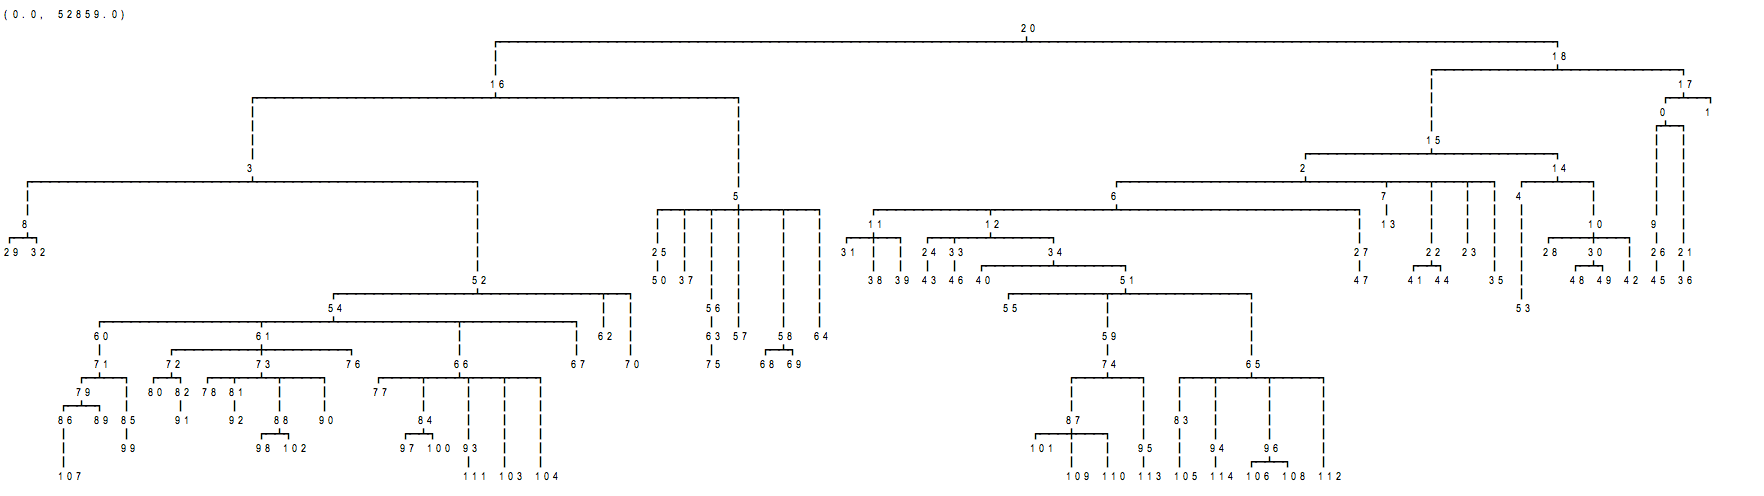
\includegraphics[width=1.0\linewidth]{../figures/BeforeSimplification}\label{fig:f1}}
  	\hfill
  	\subfloat[Simplified]{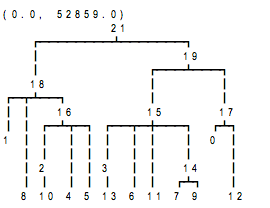
\includegraphics[width=0.15\linewidth]{../figures/AfterSimplification}\label{fig:f2}}
  	\caption{The above shows an example a of single gene tree
	within the embellished pedigree of 
	a population simulated in a SLiM non-Wright Fischer model, defined on the interval [0,52859).
	The tree was build and printed by the \textbf{msprime} succinct tree sequence Python API.
	Tree (a) was simplified to represent the genealogical histories of all extant individuals 
	which resulted in tree (b).
	With possibly hundreds of thousands of these trees defined on separate gene segments,
	it should be clear that the number of neutral mutations needed to be simulated without simplification is 
	much greater than after.
	}
   \end{center}
\end{figure}

\subsection{Succinct Tree Sequence Data Structures in msprime}

The simplification and storage of the embellished pedigree
was made possible by \textit{succinct tree sequences},
introduced by \textbf{msprime} \cite{Kelleher2016}.
These data structures store the correlated histories between sets of sampled individuals 
and are close to optimal in terms 
of algorithmic complexity and space.
Succinct tree sequences are crucial for the genealogical tree sequencing strategy 
because they allow us to efficiently insert information, simplify, and reconstruct gene trees.
For the purposes of the implementation in SLiM,
we use four primary tables.

(1) The Node table, in which each row represents a single genome within a diploid individual.
The information stored in this table is primarily the birth time of the genome as well as the population ID to which the individual belongs. 
Conceptually, this table is needed for the reference of parent-child relationships when inherited genomic intervals are recorded in the Edge table. 
Keeping the ID of the individual equivalent to its' index in the table allows for quick access of
individual for sorting, simplifying, and building tree sequences. 

(2) The Edge table is used to store each genomic interval [left, right),
where left and right are genomic locations of two breakpoints. 
In addition, it needs to store the parental genome who passed each interval down, and the offspring who inherited it. 
Because there is often quite a bit of overlap 
between trees defined on intervals which are close in proximity along the genome,
keeping the edges separate from the individuals (and the IDs of nodes mutable by index)
allows correlated trees within the embellished pedigree to share edges.

Given the Node and Edges tables, we can reconstruct a gene tree at any given location, $X$,
along the genome. 
This is because edges record the intervals at which a genome inherits from an
ancestor, so we can simply use all edges, and their respective nodes, such that $X  \in [left:right)$ to rebuild the tree at that location.

(3 and 4) Optionally, the Mutation and Sites tables are then used to record any non-neutral mutations 
that are being tracked so that the origin of those mutations are recorded within the succinct tree sequence.
This will efficiently give us the genotype\footnote{the mutation state of all positions along the genome} information for any node in the tree.
The Site table includes the position and the ancestral state so that if no mutation occurs at that location further down the lineage,
all nodes will inherit that state.
The Mutation table then records the derived state, the site, and the first node to have that mutation. 
Then, all nodes in the subtree below that node will inherit the same mutation at that position unless 
another mutation occurs.

The pruning algorithm which simplifies the trees can be vaguely described through a simple ``paint pot'' explanation.
 (1) paint each sample genome a unique color, follow each lineage back in time,
 giving the intervals inherited from each parent the respective color.
 (2) Whenever two colors merge in the same spot on an ancestor,
 record a coalescence and (3) paint the overlapped colors an entirely new color before continuing \cite{Ralph2018}. 
 This is quite oversimplified and does not include all details and edge cases,
 but explains the core properties of the algorithm.

\section{Analysis}

For an analysis of our implementation, we will look at the comparison of genealogical tree sequence recording in contrast to simulating neutral mutations. 
We use runtime as our primary performance measure but also look at memory usage.
In two separate model types, we observed large performance gains. 
In trivial model comparisons, genealogical tree sequence recording reduced runtimes by approximately two orders of magnitude. 
For more realistic model comparisons, we observed 24X speedup.

For \textit{all} simulations with tree sequence recording, we retroactively laid neutral mutations over the trees at the same mutation rate using msprime. 
We then added the time it took to the runtime of the simulations.
This was to ensure all simulations produced statistically equivalent results.

%TODO: LARGER RUNTIMES COMING
%FEEDBACK ON FIGURES?

\subsection{Neutral Model Benchmark Simulations}

First, we compare trivial models in which all mutations are neutral.
This gives us a baseline of the performance difference between the two strategies
as tracking mutations is the heaviest consumer of the computation time.
The neutral model also allows us to compare our simulations to a coalescent in msprime,
given that they do not violate the 
Markovian process\footnote{the conditional probability distribution of future states of the process 
(conditional on both past and present states) depends only upon the present state, 
not on the sequence of events that preceded it.}
A fixed mutation and recombination rate allow for us to compare the models as their magnitude is 
scaled by the length of the chromosome from $10^{5}$ to $10^{10}$. 
The models have 500 diploid\footnote{having two sets of homologous chromosomes} 
individuals (so N=Ne=1000 in msprime), 
mutation rate of $10^{-7}$ (or 0, when doing TreeSeq), and a recombination rate of $10^{-8}$.  
All simulations were run for 5000 generations and 
the size of the genome was scaled to increase the total amount of work.

%\todo[inline]{Instead of hard-coding figure numbers, use distinct labels in figures and then refer to them with ref and place figures near the relevant text -- this allows latex to optimize figure placement.}

In Figure \ref{fig:NeutralComp}, we can see that the genealogical tree sequence recording has no performance gain until the length
of the chromosome reaches $10^{7}$. After approaching realistic size genomes $10^{8}$, 
we start to see pedigree run just under two orders of magnitude faster compared to simulating neutral mutations throughout. 
Unexpectedly, at $10^{10}$ scaled chromosome lengths,
the forward-moving simulation runtime was less than its coalescent counterpart's runtime for all sample sizes.
It is unclear whether this is a result of the nature of the simulations 
or simply a difference in the implementations. 


\begin{figure}[h!tb]
	\begin{center}
  		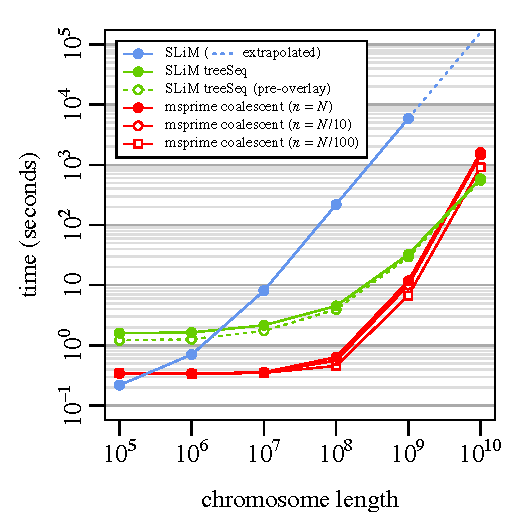
\includegraphics[width=0.7\linewidth]{../figures/comparison.pdf}
  		\caption{
		Total runtime as a function of chromosome length in each simulation. 
		This chart shows SLiM tracking neutral mutations (Blue),
		SLiM with genealogical tree sequence recording (Green), and msprime coalescent (Red)
		with different sample sizes. 
		Plotted on a log scale we can see the scalability 
		of the genealogical tree sequence recording strategy as it reduces runtime 
		by over two orders of magnitude for realistic size genomes.
		}
  		\label{fig:NeutralComp}
	\end{center}
\end{figure}




\subsection{Non-Neutral Benchmark Simulations}

Next, we reproduce the simulation benchmarks done with the simulation frameworks fwdpp in \cite{Ralph2018}.
These models represent how more realistic forward-moving simulations behave under selection. 
Thousands of deleterious\footnote{mutations which are harmful to an individuals fitness}
mutations are introduced and acted upon by selection.
As selected mutations impact the outcome of the simulation,
TreeSeq must track them throughout the simulation run for every genome that carries a deleterious mutation type.
Therefore, all time savings from TreeSeq come directly from not tracking neutral mutations throughout.
Furthermore, the selection on multiple mutations is a violation of the exchangeability assumptions of the coalescent,
meaning regressive simulations cannot recreate this model and the trees they create are novel.

Each simulation was a Wright-Fisher model with $N$ individuals and ran for a total of $10N$ generations.
$\rho$ is an estimation of the total amount of work to be done in the simulation
as it represents twice the number recombination events per generation.
The size ($\rho$) of the simulations was increased over two separate values of $N$
to observe the scalability of this strategy.
recombination and mutation rates were each set to $\rho / 4N / 10^{8}$, where $10^{8}$ was the total number of 
loci\footnote{abstraction of a position along the genome} 
per genome. 
The number of new mutations and breakpoints\footnote{a breakpoint is the position on the chromosome that breaks 
during meiosis before recombining with its homologous chromosome}
per diploid, per generation, were equivalent. 

\begin{figure}[h!tb]
	\begin{center}
  		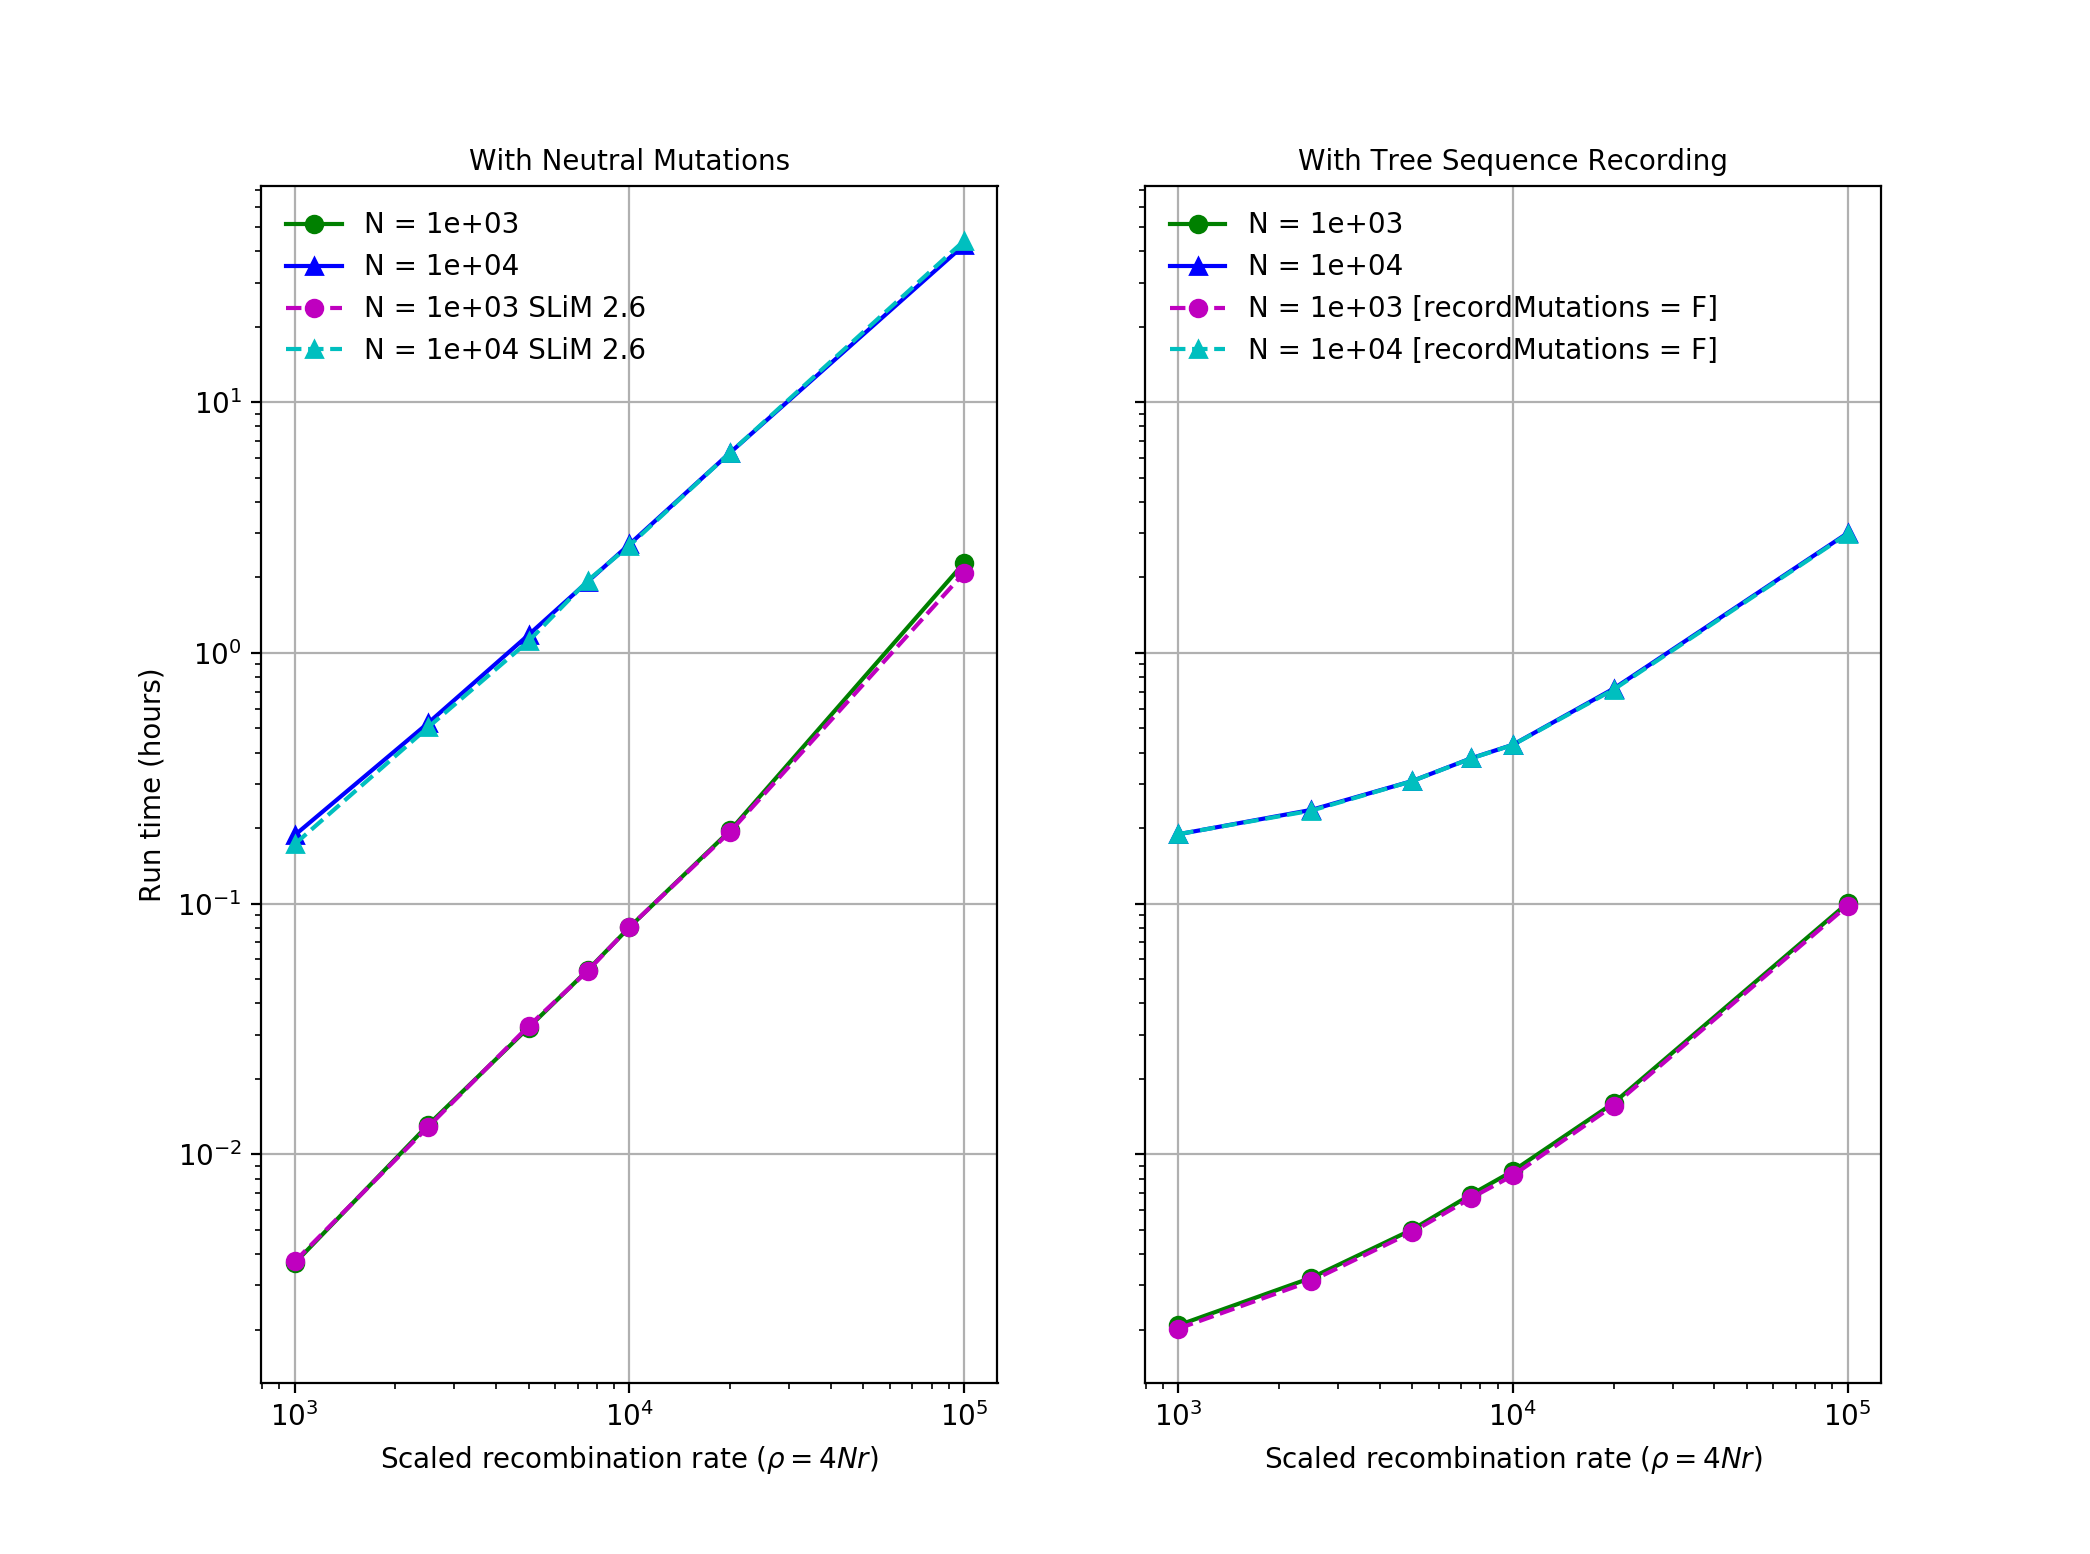
\includegraphics[width=1.0\linewidth]{../figures/RuntimeLog.png}
  		\caption{
		Total runtime as a function of $\rho = 4Nr$, where r is the effective recombination rate.
		All simulations were run with two different values of population size ($N$) to observe scaling of number of individuals.
		On the left we can see the runtimes for SLiM tracking all neutral mutations 
		and not recording the genealogical tree sequence.
		The dashed pink and light blue were run with the stable release version of SLiM 2.6.
		On the right, we show the same simulations run with genealogical tree sequence recording and laying 
		neutral mutations over the trees retroactively.
		Here, dashed pink and light blue represent genealogical tree sequence recording with the $[record mutations = F]$ option. 
		}
  		\label{fig:NonNeutralComp}
	\end{center}
\end{figure}


As can be seen in Figure \ref{fig:NonNeutralComp}, pedigree recording on non-neutral models reduced runtimes dramatically.
With $\rho = 10^{5}$, for both sizes of $N$, we saw 10-fold time savings.
The largest savings were seen at parameter values $N = 10^{3}$ and $\rho = 10^{5}$,
where tracking neutral mutations ran in $8230.91$ seconds and TreeSeq only took $354.78$ second
resulting in a $23.2X$ speedup. 
At $N = 10^{4}$ and $\rho = 10^{5}$,
tracking neutral mutations ran in $8230.91$ seconds in comparison to TreeSeq which only took $354.78$ seconds,
giving a $14.17X$ speedup. 

\begin{figure}[h!tb]
	\begin{center}
  		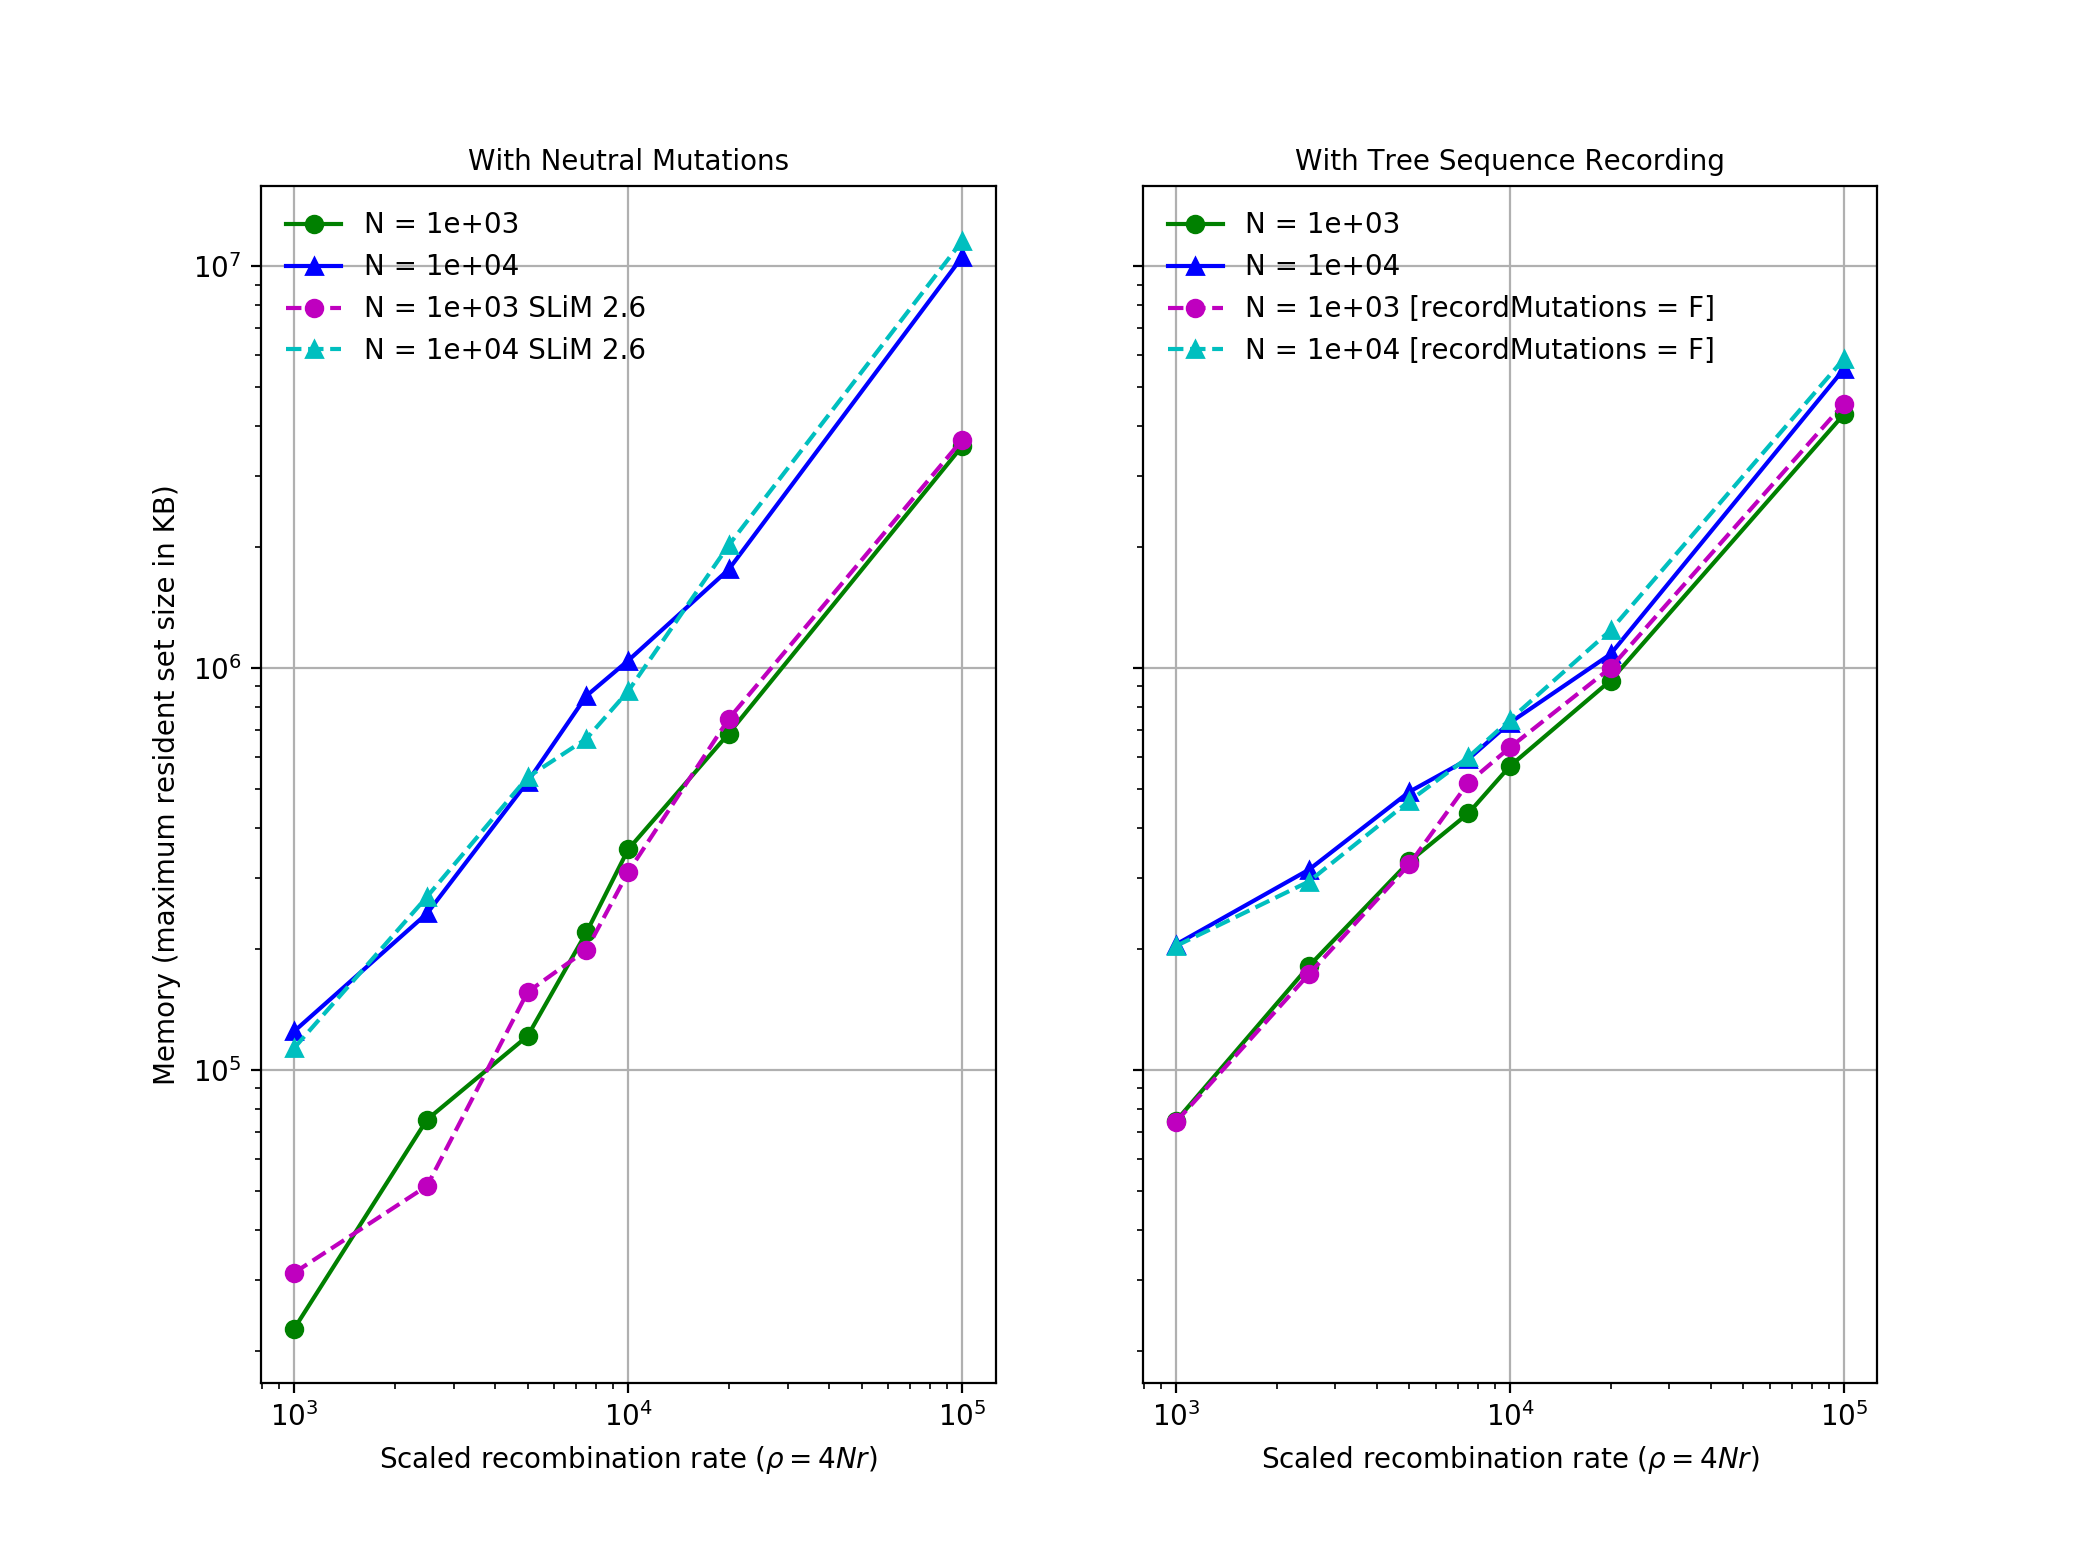
\includegraphics[width=1.0\linewidth]{../figures/MemoryLog.png}
  		\caption{
		Total memory (maximum resident set size in KB) as a function of $\rho = 4Nr$, where r is the effective recombination rate.
		All simulations were run with two different values of population size ($N$) to observe scaling of number of individuals.
		On the left we can see the memory for SLiM tracking all neutral mutations 
		and not recording the genealogical tree sequence.
		The dashed pink and light blue were run with the stable release version of SLiM 2.6.
		On the right, we show the same simulations run with genealogical tree sequence recording and retroactively laying 
		neutral mutations over the trees.
		Here, dashed pink and light blue represent genealogical tree sequence recording with the $[recordMutations = F]$ option. 
		}
  		\label{fig:NonNeutralMemComp}
	\end{center}
\end{figure}



For smaller simulations, TreeSeq took a larger amount of memory when compared to tracking neutral mutations. 
This is relatively unsurprising when you consider that we're tracking the simplified genealogical history of all individuals throughout the simulation.
Impressively, as seen in Figure \ref{fig:NonNeutralMemComp}, we observed memory savings at larger parameter values.
This illustrates that tracking the accumulation of neutral mutations in large population sizes becomes more of a burden on RAM compared 
to storing the genotype origins. 
For $N = 10^{4}$ and $\rho = 10^{5}$, tracking neutral mutations had nearly twice the resident size in KB.

It's important to note the speed-memory tradeoff that is made when deciding how often to simplify the tables.
If the user were to simplify the tables very frequently, the implementation would require less memory due to the smaller average size of tables,
yet it would run slower because of the computation required in simplification.
Alternatively, infrequent simplification would cause the tables to grow large and require more memory. 
Here, we measure the ratio of the tables before and after each simplification to determine when to simplify next.
By default, the ratio is set to 10; meaning we adjust the simplification interval such that the size of the tables 
after simplification is $\approx 1/10^{th}$ of the table sizes before simplification.

The TreeSeq implementation optionally includes the ability to record mutations ($[recordMutations = T]$) in the 
\textit{sites} and \textit{mutations} tables as part of the succinct tree sequence.
For all TreeSeq simulations, the difference in runtime using this feature was trivial.
This is exciting because tracking the selected mutations in the gene trees gives us
insight into the origins of genotypes and tree dynamics under the influence of evolutionary forces.

\section{SLiM TreeSeq Implementation}

Conceptually, this implementation uses the conjunction of SLiM and msprime  
to easily allow the investigation of a large number of dynamics surrounding gene trees generated through large,
forward-moving simulations with a very straitforward workflow:
(1) Create any model which you would like to study in 
SLiM and simply flip a switch in the initialize block which tells SLiM to record the embellished pedigree |
keeping in mind the model does not need to include neutral mutations, 
which allows much less strict constraints on the magnitude of simulations.
(2) Import the tables file generated by SLiM, and load it into the msprime Python API 
to gain access to a large number of analysis tools.

More Specifically, the user is simply able to add 
a single line of code to their SLiM model with the following function signature:
\begin{lstlisting}[basicstyle=\small,] 
(void) initializeTreeSeq( 
  [logical$ recordMutations = T], 
  [float$ simplificationRatio = 10], 
  [logical$ checkCoalescence = F], 
  [logical$ runCrossChecks = F]); 

\end{lstlisting} 
This tells SLiM to record the embellished pedigree
into the succinct tree sequence, as well as periodically simplify on samples and extant individuals throughout the simulation run.
When the user would like to access the tables for analysis,
they can then simply add
\begin{lstlisting}[basicstyle=\small,] 
(void) sim.treeSeqOutput(
  string$ path,
  [logical$ simplify = T]);

\end{lstlisting} 
to write the tables file either in text or binary at any given generation. 
The tables file, compatible with \textbf{msprime} python API allows the user to easily lay neutral mutations over the trees, 
compute statistics, or even run a coalescent simulation on top of the trees to complete
the history. 

\subsection{Pseudo Code}

Here, we will describe the initial proof-of-concept implementation. 
This describes what was done initially to
record the genealogical history (Nodes and Edges) from the internal
source code of SLiM
into the tables code found in \textbf{msprime}.
the C code was isolated into it's own API so that we could compile it with SLiM.
The following are the core function signatures called from within SLiM. 
\vspace{25mm} %5mm vertical space
\begin{algorithmic}[1]

\Procedure{nodeTableAddRow}{}
\State $\textit{Self} \gets \text{Reference to }\textit{NodeTable}\text{ being added to}$
\State $\textit{Time} \gets \text{Generation that the Genome was born}$
\State $\textit{Population} \gets \text{Reference to subpopulation genome was born in}$
\EndProcedure

\Procedure{edgeTableAddRow}{}
\State $\textit{Self} \gets \text{Reference to }\textit{EdgeTable}\text{ being added to}$
\State $\textit{Left} \gets \text{Left hand side of Genomic Interval, }\textit{closed} $
\State $\textit{Right} \gets \text{Right hand side of Genomic Interval, }\textit{open} $
\State $\textit{Parent} \gets \text{msprime Node id (index) of Parent Node}$
\State $\textit{Child} \gets \text{msprime Node id (index) of Offspring Node}$
\EndProcedure

\Procedure{sortTables}{}
\State $\textit{Nodes} \gets \text{Reference to }\textit{NodeTable}$
\State $\textit{Edges} \gets \text{Reference to }\textit{EdgeTable}$
\EndProcedure

\Procedure{simplifyTables}{}
\State $\textit{Nodes} \gets \text{Reference to }\textit{NodeTable}$
\State $\textit{Edges} \gets \text{Reference to }\textit{EdgeTable}$
\EndProcedure

\end{algorithmic}
\vspace{5mm} %5mm vertical space

\begin{algorithm}
\algdef{SE}[SUBALG]{Indent}{EndIndent}{}{\algorithmicend\ }%
\algtext*{Indent}
\algtext*{EndIndent}
\caption{Genealogical Tree Sequence Recording}\label{euclid}
\begin{algorithmic}[1]
\item\textbf{\#include}\text{ msprime}\textbf{ as}\text{ msp}
\item\textbf{member}\text{NodeTable}
\item\textbf{member}\text{EdgeTable}
\item\textbf{member}\text{MspidMAP}
\Procedure{RecordNewGenome}{}
\State $\textit{breakpoints} \gets \text{vector of genomic intervals inherited from each parent}$
\State $\textit{parent} \gets \text{pointer to parental individual}$
\BState \emph{top}:
\State $\textit{time} \gets -1 * \text{currentGeneration}$
\State $\textit{offSpringMSPID} \gets \Call{msp.nodeTableAddRow}{NodeTable,time,newGenome}$
\State $\textit{newGenome.MSPID} \gets \textit{offspringMSPID}$
\State $\textit{genome1MSPID} \gets  \textit{MspidMAP} [ \textit{parent.pedigreeID} * 2] $
\State $\textit{genome2MSPID} \gets  \textit{MspidMAP} [ genome1MSPID + 1] $
\State $\textit{left} \gets 0.0$
\State $\textit{polarity} \gets \text{TRUE}$
\State for $k = 0$, $k{+}{+}$, while $k < breakpoints.size()$
\Indent
\State $\textit{right} \gets \textit{breakpoints}[k]$
\State $\textit{parent} \gets \textit{polarity } ? \textit{ genome1MSPID } : \textit{ genome2MSPID}$
\State $\Call{msp.edgeTableAddRow}{left,right,parent,offspringMSPID}$
\State $\textit{left} \gets \textit{right}$
\State $\textit{polarity} \gets \textit{! polarity}$
\EndIndent	
\State $\textit{right} \gets \textit{chromosome.lastPosition} + 1$
\State $\textit{parent} \gets \textit{polarity } ? \textit{ genome1MSPID } : \textit{ genome2MSPID}$
\State $\Call{msp.EdgeTableAddRow}{left,right,parent,offspringMSPID}$
\EndProcedure

\Procedure{Simplify}{}
\BState \emph{top}:
\State $\textit{Samples} \gets []$
\State $\textit{newMap} \gets [:]$
\State $\textit{newGenomeMSPID} \gets 0$
\State for $ind$ in $extantIndividuals$:
\Indent
\State $\textit{g1} \gets ind.pedigreeID * 2$ 
\State $\textit{g2} \gets g1 + 1$ 
\State $\textit{Samples.append}(MspidMap[g1])$
\State $\textit{Samples.append}(MspidMap[g2])$
\State $\textit{MspidMap}[g1] \gets \textit{newGenomeMSPID}{+}{+}$
\State $\textit{MspidMap}[g2] \gets \textit{newGenomeMSPID}{+}{+}$
\EndIndent
\State \Call{msp.sortTables}{Nodes,Edges}
\State \Call{msp.simplifyTables}{Nodes,Edges}
\State MspidMap = newMap

\EndProcedure

\end{algorithmic}
\end{algorithm}

To record the embellished pedigree, we needed to record all new genomes being generated, 
as well as the parent-child relationships of each genomic interval being passed down.
In terms of the code that needed to be added, we needed
(1) a method that was called (In Eidos) when the user initialized tree recording
(2) a method that was called for each recombination event (twice directly after each individual was created), giving us a vector of all breakpoints.
(3) a method to simplify the tables against the set of all extant individuals and samples.
(4) a method that was called (In Eidos) when the user wants to write out the tree sequences. \

When recording a node and it's respective edges, conceptually, we are recording the result of a meioses event in which 
gametes \footnote{sex cells} produce 
germ cells \footnote{a cell containing one genome to be recombined with a germ cell of the opposite sex containing the homologous set of chromosomes, such as a sperm or an egg}
Each individual in the SLiM simulation has a unique ID and each individual has two genomes.
Consequently, to keep an original genome ID with reference to the individual who possesses it,
we decided to follow the heuristic

\begin{center}
individual.genome1.id = individual.id * 2,
and,

individual.genome2.id = individual.id * 2 + 1.
\end{center}

Given this information, the implementation just needed to loop through the breakpoints 
and give the correct nodes and edges to the msprime API so it could record the data.
Once the correct information from the simulation was recorded into the tables, 
we needed to periodically simplify the tables so they don't grow too big. 

SLiM individual ID's were fixed and generated sequentially throughout the simulation.
In contrast, msprime node IDs are dynamically kept as their index into the tables.
One complication with this was referencing parent-child relationships when adding edges.
Up to the first simplification, these IDs would be identical.
However, one consequence of the simplification algorithm was that all sampled individuals which were being simplified against
would be moved to the top of the table, changing their respective ID in msprime. 
consequently, we had to map SLiM IDs to msprime node IDs for each simplification.
In Algorithm 1, we can see the pseudo-code for (2) RecordNewGenome and (3) Simplify. 


\subsection{Algorithm and Data Structure Improvements}

A bottleneck for our implementation was the mapping of genome IDs in SLiM to node IDs 
in the msprime tables code.
In certain simulations, the re-mapping insertion and key-value searches could take up $40\%$ of the entire simulation runtime. 
The consistent use of the map
was due to genomic intervals (edges) being recorded to the edge table.
Each edge needs access to the msprime id of the parent passing down that value.

Our initial map was implemented as a red-black tree where
each internal node was a unique key (SLiM Genome ID) containing its respective value (msprime node).
This data structure is similar to a binary search tree, providing an ordered representation of the data it holds. 
Balancing the tree through a method of subtree rotations at time of insertion guarantees that 
the height of the tree will remain $2\log_2{n+1}$ given n nodes in the tree.
As a result of this tree height, 
each search and insertion into the map was completed in $O(\log{}n)$ time where n 
was the existing number of entries into the tree. 

For every simplification, we needed two entries per individual into the map,
Then for every genome recorded afterward, 
we needed two additional searches into the map. 
This resulted in a time complexity of $O(n\log{}n)$ yet a large constant from heavy use make it very inefficient. 
Ordered data structures like this tend to be more efficient when there are
fewer entries in the table. 
In our case, large simulations could lead to potentially hundreds of thousands
of entries into the tables.

Fortunately, the use of an ordered data structure was not necessary for our implementation.
So our first step to optimizing this bottleneck was to replace the red-black tree with a hash table. 
A hash table can be thought of as an array of 'buckets', each having a unique hash value representing the 
'hash' of a range of the keys inserted into the tables. Each bucket is essentially a linked
list data structure which contains the key-value pairs. 
% a tree is better for smaller.

To add a key-value pair to the table simply apply the hash function to the key,
index to the respective hash bucket,
and insert the value at the end of the table. 
a search for the key-value is then a similar process of hashing the key and doing a linear search through the bucket until the value is found.
The amortized complexity of search, insert, and removal, is $O(1)$. 

%reference the algorithm!

This method of using an unordered map allowed for a significant
increase in speed. Using the $\rho$ benchmark model as a comparison between the two data structure implementations, we found that using an unordered map sped up the initial a genealogical tree sequence recording simulation by $20\%$.

Initially, our use of these data structures was to try and keep the implementation from messing with SLiM's core code. 
However, keeping a reference to the msprime 
node ID directly with the genome objects, 
would eliminate the need for an external data structure.
Furthermore, we were already doing the 
necessary computations to reassign these values in SimplifyTables().
Keeping reference directly with the genome objects resulted in 
some non-trivial time savings as well as simplifying the code

Below we show a table of the run times for each implementation using the same simulations seen in Figure 3 for the non-neutral, genealogical tree sequence recording model at parameter values N = $10^{4}$ and $\rho$ = $10^{4}$. 
We compare the runtimes of an ordered map, unordered map, and keeping the reference directly with the genome objects. 


\vspace{5mm} %5mm vertical space
\begin{tabular}{ |p{2.2cm}||p{2.2cm}|p{2.2cm}|p{2.2cm}|  }
 \hline
 \multicolumn{4}{|c|}{Runtime Performance Gain} \\
 \hline
 Implimentation  & runtime \newline (seconds) & speedup from Neutral & speedup from Initial\\
 \hline
Neutral Muts   & $9942.8$ & -- &  --\\
Red-Black  & $2593.5$ & $3.84X$ & --\\
Hash & $2091.4$ & $5.75X$ & $1.24X$\\
Reference & $1549.0$ & $6.418X$ & $1.67X$\\

 \hline
\end{tabular}

\newpage

\begin{comment}

\section{An application of TreeSeq}

%show a comparison graph of stickleback model to show that 
%genealogical tree sequence recording and neutral mutations are identical 
%WAITING ON RESULTS TO FINISH THIS SECTION

To give you an idea about the use of our implementation, we will now 
provide a practical application of genealogical tree sequence recording. 
Will will apply the implementation to a simulation model used for the study of 
rapid and parallel adaptation of marine stickleback fish to freshwater environments.
This is a model 



\subsection{Stickleback Research}

\begin{figure}
	\begin{center}
  		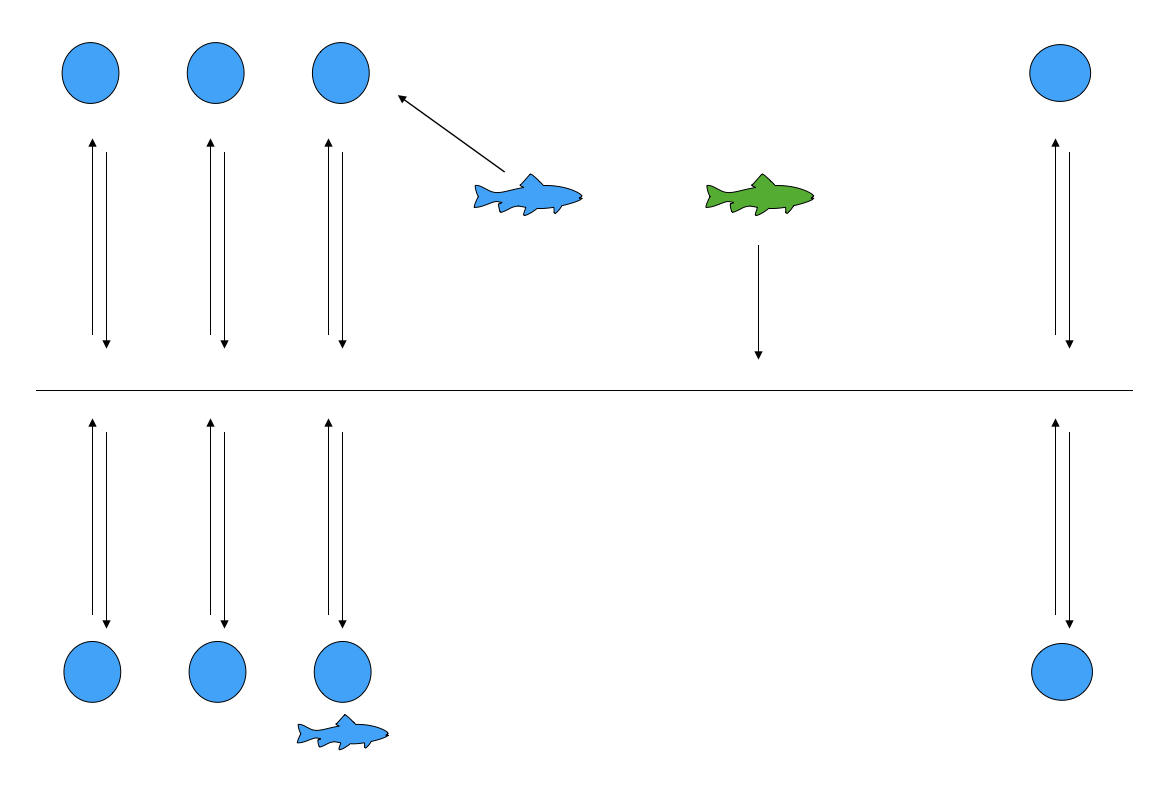
\includegraphics[width=0.7\linewidth]{SticklebackGeography}
  		\caption{
		This diagram represents the geographic layout of the stickleback model. 
		The line emulates a coastal marine population of stickleback in a one-dimensional continuous space - 
		connected to many, much smaller discrete freshwater populations of stickleback. 
		Continuous space is one limitation in regressive simulation models such as coalescence theory, 
		Consequently, recording the embellished pedigree in a model like this for large simulations has not been possible 
		without this strategy. 
		}
  		\label{fig:boat1}
	\end{center}
\end{figure}

One major question in ecology involves studying the rapid and parallel adaptation of species.
Using forward moving simulations, 
We can emulate the the geography, selective pressure, and genomic architecture
of Threespine Stickleback populations in Alaska to better understand the data we observe in nature.
Figure \ref{fig:boat1} shows the complex geographic setting of the stickleback model which is 
modeled using \textbf{SLiM 2}. \todo{comparison.pdf not in repo, also duplicate label fig:boat1}
The hypothesis behind rapid and parallel adaptation is that stickleback in marine populations carry 
freshwater alleles that are able to be selected upon when marine individuals inhabit a new freshwater environment.
to fully understand the origins of genomic variation among the populations we can use the tree sequence and look at 

\subsection{Results of Genealogical Tree Sequence Recording}

\end{comment}

\section{Conclusions and Future Work}

This paper covers the basics of genealogical tree sequence recording and the core of its implementation SLiM. 
We have shown that this method results in large performance in gains in runtime and even memory after at large parameter values.
Additionally, we have conveyed how genealogical tree sequence recording
opens the door to a wide range of theoretical population genetics research surrounding gene trees
through the use of forward-moving evolutionary simulations.
We have shown how the general public can make use of this implementation and the core of it's implementation.
Finally, we have explored the optimizations that make this strategy even faster. 

It should be noted that the remaining bottleneck in out implementation
lies with having to sort the tables before each simplification. 
Given the nature of the tables and the algorithm for recording/simplifying them, 
a (possibly large) portion of the edge table remains sorted between simplification intervals. 
The portion of the tables up to the oldest individual in the last simplification
does not need to be re-sorted as the individuals cannot possibly be parents to the generation of offspring following simplification.
This implies that we could potentially save computation by sorting only the necessary portions of the tables.
Unfortunately, the implementation of the tables API was created for regressive simulations, 
meaning the order the tables are sorted in makes this optimization much less trivial, but not impossible. 

This paper highlights the most fundamental aspects of implementing tree sequence recording.
In contrast, it fails to explore the detail and complexity of the actual code put into SLiM that will be available to the public. 
Peter Ralph, Ben Haller, and Jerome Keller and I have put a large amount of work into testing, extending user features,
optimizations, and making genealogical tree sequence recording receptive to the flexibility of SLiM.  

\newpage


\bibliography{Citations}{}
\bibliographystyle{plain}
\newpage

\section{Code for Examples and Figures}

%\todo{Add a short description here}
Here, we provide the code for all simulations run in analysis section,
the optimized code from the improved data structures, 
and the msprime code used to read in tree files. 
Additional bash scripts, raw data, and msprime python code 
can be found at 
\url{https://github.com/jgallowa07/SLiM_TSBenchmarks}
The source code for this paper can be found at 
\url{https://github.com/jgallowa07/UndergraduateThesis}

\newpage
\subsection{Algorithm with Optimizations}

\begin{algorithm}
\algdef{SE}[SUBALG]{Indent}{EndIndent}{}{\algorithmicend\ }%
\algtext*{Indent}
\algtext*{EndIndent}
\caption{Genealogical Tree Sequence Recording Algorithm}\label{euclid}
\begin{algorithmic}[1]
\item\textbf{member}\text{NodeTable}
\item\textbf{member}\text{EdgeTable}
\Procedure{RecordNewGenome}{}
\State $\textit{breakpoints} \gets \text{vector of genomic intervals inherited from each parent}$
\State $\textit{newGenome} \gets \text{a pointer to the genome object being created}$
\State $\textit{parent1} \gets \text{pointer to initial parental genome}$
\State $\textit{parent2} \gets \text{pointer to second parental genome}$
\BState \emph{top}:
\State $\textit{time} \gets -1 * \text{currentGeneration}$
\State $\textit{offSpringMSPID} \gets \Call{nodeTableAddRow}{NodeTable,time,newGenome}$
\State $\textit{newGenome.MSPID} \gets \textit{offspringMSPID}$
\State $\textit{genome1MSPID} \gets  \textit{parent1.MSPID}$
\State $\textit{genome2 MSPID} \gets \textit{(!parent2) ? genome1MSPID : parent2.MSPID}$
\State $\textit{left} \gets 0.0$
\State $\textit{polarity} \gets \text{TRUE}$
\State for $k = 0$, $k{+}{+}$, while $k < breakpoints.size()$
\Indent
\State $\textit{right} \gets \textit{breakpoints}[k]$
\State $\textit{parent} \gets \textit{polarity } ? \textit{ genome1MSPID } : \textit{ genome2MSPID}$
\State $\Call{edgeTableAddRow}{left,right,parent,offspringMSPID}$
\State $\textit{left} \gets \textit{right}$
\State $\textit{polarity} \gets \textit{! polarity}$
\EndIndent	
\State $\textit{right} \gets \textit{chromosome.lastPosition} + 1$
\State $\textit{parent} \gets \textit{polarity } ? \textit{ genome1MSPID } : \textit{ genome2MSPID}$
\State $\Call{EdgeTableAddRow}{left,right,parent,offspringMSPID}$
\EndProcedure

\Procedure{Simplify}{}
\BState \emph{top}:
\State $\textit{Samples} \gets []$
\State $\textit{newGenomeMSPID} \gets 0$
\State for $g$ in $extantGenomes$:
\Indent
\State $\textit{Samples.append}(g.MSPID)$
\State $\textit{g.MSPID} \gets \textit{newGenomeMSPID}{+}{+}$
\EndIndent
\State \Call{sortTables}{Nodes,Edges}
\State \Call{simplifyTables}{Nodes,Edges}
\EndProcedure

\end{algorithmic}
\end{algorithm}

\newpage

\subsection{Recipe for Figure 1}

\begin{lstlisting}[basicstyle=\small,]

initialize(){
	setSeed(1523562691046);
	initializeSLiMModelType("nonWF");
	initializeTreeSeq(runCrosschecks=T);
	defineConstant("K", 5);
	initializeMutationType("m1", 0.5, "f", 0.0);
	m1.convertToSubstitution = T;
	initializeGenomicElementType("g1", m1, 1.0);
	initializeGenomicElement(g1, 0, 99999);
	initializeMutationRate(1e-7);
	initializeRecombinationRate(1e-8);
}
reproduction()
{
	subpop.addCrossed(individual, subpop.sampleIndividuals(1));
	return NULL;
}
1 early()
{
	sim.addSubpop("p1", 5);
}
early()
{
	p1.fitnessScaling = K / p1.individualCount;
}
10 late()
{

	sim.treeSeqOutput("~/Documents/UndergraduateThesis/ \
		UnsimplifiedTable/",binary = F,simplify = F);
	sim.treeSeqOutput("~/Documents/UndergraduateThesis/ \
		SimplifiedTable/",binary = F,simplify = T);
	sim.simulationFinished();

}

\end{lstlisting}

\newpage

\subsection{msprime code tree printing}
\begin{lstlisting}[basicstyle=\small,]

from testutils import *
import sys
import io
#/Users/jaredgalloway/Documents/UndergraduateThesis/UnsimplifiedTable
nodes_U = open("/UnsimplifiedTable/NodeTable.txt","r")
edges_U = open("/UnsimplifiedTable/EdgeTable.txt","r")
mutations_U = open("/UnsimplifiedTable/MutationTable.txt","r")
sites_U = open("UnsimplifiedTable/SiteTable.txt","r")

nodes_S = open("/SimplifiedTable/NodeTable.txt","r")
edges_S = open("/SimplifiedTable/EdgeTable.txt","r")
mutations_S = open("/SimplifiedTable/MutationTable.txt","r")
sites_S = open("/SimplifiedTable/SiteTable.txt","r")

#Nodes = msprime.parse_nodes(nodes_U,base64_metadata=False)

tr_U = msprime.load_text(nodes=nodes_U, edges=edges_U, 
		       sites=sites_U, mutations=mutations_U,
		       base64_metadata=False)

tr_S = msprime.load_text(nodes=nodes_S, edges=edges_S, 
		       sites=sites_S, mutations=mutations_S,
		       base64_metadata=False)

#print(type(tr))
unsimplified = tr_U.trees()
simplified = tr_S.trees()


for i in unsimplified:
	print(i.draw(format="unicode"))
	print(i.interval)

for i in simplified:
	print(i.draw(format="unicode"))
	print(i.interval)

\end{lstlisting}

\newpage

\subsection{Recipes for Neutral Simulations}

\begin{lstlisting}[basicstyle=\small,]
initialize() {
    catn("Seed == " + getSeed());
    catn("L == " + Lstr);
    catn("OUTFILE == " + OUTFILE);
    catn();
    
    defineConstant("L", asInteger(Lstr));
    
    initializeMutationRate(1e-7);
    initializeMutationType("m1", 0.5, "f", 0.0);
    initializeGenomicElementType("g1", m1, 1.0);
    initializeGenomicElement(g1, 0, L-1);
    initializeRecombinationRate(1e-8);
}
1 {
    sim.addSubpop("p1", 500);
}
5000 late() {
    sim.outputFull("./output/"+OUTFILE, binary=T);
}

\end{lstlisting}


\subsection{Recipes for Non-Neutral Simulations}

\begin{lstlisting}[basicstyle=\small,]
//---------neutral models---------
initialize() {
	N = n_ind;
	rho = size_rho;
	numLoci = 1e8;
	r = rho / (4*N);
	mutation_recombination_Rate = r / numLoci; 
	defineConstant("NumInd",N);
    	initializeMutationRate(mutation_recombination_Rate);
    	//Neutral Mutations
	initializeMutationType("m1", 0.5, "f", 0.0);
	//Deleterious Mutations
    	initializeMutationType("m2", 0.5, "g", -5 / (2*N), 1.0);	
    	initializeGenomicElementType("g1", c(m1,m2), c(99.0,1.0));
    	initializeGenomicElement(g1, 0, numLoci-1);
    	initializeRecombinationRate(mutation_recombination_Rate);	
}
1 late() { sim.addSubpop("p1", NumInd); 
	timeToRun = 10 * NumInd;
	sim.rescheduleScriptBlock(s1,timeToRun,timeToRun);
}
s1 10000 late() { 
	catn("Simulation Finished");
	sim.simulationFinished(); 
}

// ---------treeSeq Models------------

initialize() {	
	initializeTreeSeq();
    	N = n_ind;
    	rho = size_rho;
    	numLoci = 1e8;
    	r = rho / (4*N);
    	mutation_recombination_Rate = r / numLoci; 
    	defineConstant("NumInd",N);
    	initializeMutationRate(mutation_recombination_Rate / 100);
	//Deleterious Mutations (only)
    	initializeMutationType("m1", 0.5, "g", -5 / (2*N), 1.0);	
    	initializeGenomicElementType("g1",m1, 1.0);
    	initializeGenomicElement(g1, 0, numLoci-1);
    	initializeRecombinationRate(mutation_recombination_Rate);
	
}
1 late() { 
	sim.addSubpop("p1", NumInd); 
	timeToRun = 10 * NumInd;
	sim.rescheduleScriptBlock(s1,timeToRun,timeToRun);
}
s1 10000 late() { 
	tablesfilestring = asString(n_ind) + "_" + \
		asString(size_rho) + "Tables";
	sim.treeSeqOutput("~/Documents/ \
		SLiM_TSBenchmarks/Bench/Tables/" + tablesfilestring);
	catn("Simulation Finished");
	sim.simulationFinished(); 
}
\end{lstlisting}

\begin{comment}
\subsection{}
\begin{lstlisting}[basicstyle=\small,]

#!/bin/bash

SEED=27467
#SECONDS_TO_KILL=`echo "72*60*60"|bc -l`

for N in 1000 10000
do
	for size in 1000 2500 5000 7500 10000 100000  
	do	
		
PED_OUTPUT_FILE_NAME=ped_output.N$N"."size$size".out"
PED_TIME_FILE_NAME=ped_timing.N$N"."size$size".out"
PED_ADD_TIME_FILE_NAME=ped_add_timing.N$N"."size$size".out"
PED_ADD_OUTPUT_FILE_NAME=ped_add_output.N$N"."size$size".out"
PED_TABLE_FILE=$N"_"$size"Tables"

NEUT_OUTPUT_FILE_NAME=neut_output.N$N"."size$size".out"
NEUT_TIME_FILE_NAME=neut_timing.N$N"."size$size".out"

PEDNM_OUTPUT_FILE_NAME=pedNM_output.N$N"."size$size".out"
PEDNM_TIME_FILE_NAME=pedNM_timing.N$N"."size$size".out"

REL_OUTPUT_FILE_NAME=rel_output.N$N"."size$size".out"
REL_TIME_FILE_NAME=rel_timing.N$N"."size$size".out"

MUTRATE=$(echo "scale=10; ($size / (4.0 * $N)) / 100000000.0" | bc)

#Neutral Mutations
/usr/local/Cellar/gnu-time/1.9/bin/gtime --format='%E / %S / %U / %M' \
--output="../ComparisonTimes/RealTimes/$NEUT_TIME_FILE_NAME" ../../../SLiM/bin/slim\ 
-s $SEED -d n_ind=$N -d size_rho=$size ../BenchRecipes/benchmarks_neutral.slim &>\  
../Output/Reals/$NEUT_OUTPUT_FILE_NAME

#Neutral Mutations Release SLiM
/usr/local/Cellar/gnu-time/1.9/bin/gtime --format='%E / %S / %U / %M' \
--output="../ComparisonTimes/RealTimes/$REL_TIME_FILE_NAME" ../../../SLiM2_6/bin/slim\ 
-s $SEED -d n_ind=$N -d size_rho=$size ../BenchRecipes/benchmarks_neutral.slim &>\ 
../Output/Reals/$REL_OUTPUT_FILE_NAME

#Pedigree Recording With Mutations
/usr/local/Cellar/gnu-time/1.9/bin/gtime --format='%E / %S / %U / %M' \
--output="../ComparisonTimes/RealTimes/$PED_TIME_FILE_NAME" ../../../SLiM/bin/slim\ 
-s $SEED -d n_ind=$N -d size_rho=$size ../BenchRecipes/benchmarks_pedigree.slim &>\ 
../Output/Reals/$PED_OUTPUT_FILE_NAME
		
#Time To layover neutral mutations over the trees
/usr/local/Cellar/gnu-time/1.9/bin/gtime --format="%E / %S / %U / %M" \
--output="../ComparisonTimes/RealTimes/$PED_ADD_TIME_FILE_NAME"\
/usr/local/bin/python3.6 add-mutation.py --mut_rate $MUTRATE --tree_file\
../Tables/$PED_TABLE_FILE -o ../VCF_Tables/ &> \
../Output/Reals/$PED_ADD_OUTPUT_FILE_NAME  

#Pedigree Recording W/O Mutations
/usr/local/Cellar/gnu-time/1.9/bin/gtime --format='%E / %S / %U / %M' \
--output="../ComparisonTimes/RealTimes/$PEDNM_TIME_FILE_NAME" ../../../SLiM/bin/slim \
-s $SEED -d n_ind=$N -d size_rho=$size ../BenchRecipes/benchmarks_pedigree_nm.slim &>\
../Output/Reals/$PEDNM_OUTPUT_FILE_NAME

	done
done

\end{lstlisting}

\end{comment}

\end{document}


